% TEXINPUTS=.:$HOME/git/bvtex: latexmk  -pdf <main>.tex
\documentclass[xcolor=dvipsnames]{beamer}

\input{defaults}
\input{beamer/preamble}

\setbeamertemplate{navigation symbols}{}
% \setbeamertemplate{background}[grid][step=1cm]

\usepackage{siunitx}
\usepackage{xmpmulti}
\usepackage[export]{adjustbox}

\usepackage[outline]{contour}
\usepackage{tikz}
\usetikzlibrary{shapes.geometric, arrows}
\usetikzlibrary{positioning}

\definecolor{bvtitlecolor}{rgb}{0.98, 0.92, 0.84}
\definecolor{bvoutline}{rgb}{0.1, 0.1, 0.1}

\renewcommand{\bvtitleauthor}{Brett Viren\\\small(for the Wire-Cell effort)}
\renewcommand{\bvtit}{WC\&Bee}
\renewcommand{\bvtitle}{\LARGE Bee and Wire Cell \\\Large Status and Larsoft Integration Plans}
\renewcommand{\bvevent}{DUNE Collaboration\\ \small 21 May 2016}
\renewcommand{\bvbeamerbackground}{}

\begin{document}
\input{beamer/title.tex}
\input{beamer/toc.tex}

\section{Bee}

\begin{frame}
  \frametitle{Bee in a nutshell}

  A web application for LArTPC event visualization and reconstruction
  \begin{itemize}
  \item Interactive 3D frontend through WebGL and JavaScript.
  \item Event file catalog through Django backend.
  \item Supports all major browsers including mobile devices.
  \end{itemize}

  \vspace{3mm}

  Feature highlights:
  \begin{itemize}
  \item Overlay results of multiple algorithms.
  \item MC truth overlay and particle hierarchy browser.
  \item 2D projections, sliced animation, keyboard navigations.
  \item Multiple geometries (MicroBooNE, 35t, protoDUNE, ...).
  \item User file upload through drag\&drop.
  \end{itemize}
\end{frame}

\begin{frame}
  \frametitle{Seeing is Bee-lieving}
  
    \begin{center}
      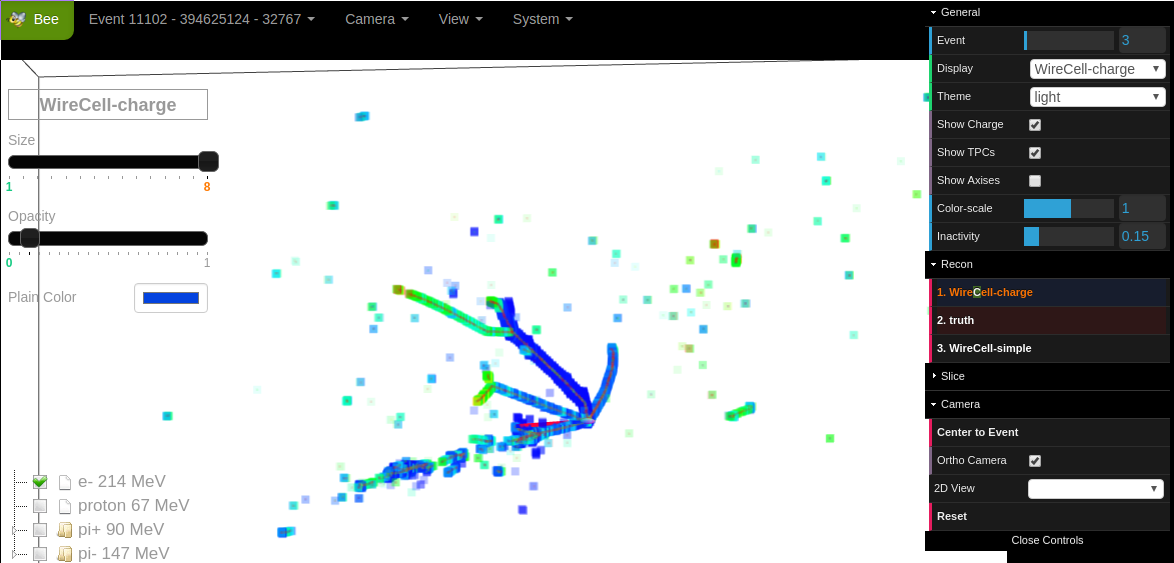
\includegraphics[width=0.9\textwidth]{bee.png}

      \vspace{5mm}

      \url{http://www.phy.bnl.gov/wire-cell/bee/}
    \end{center}

\end{frame}

\begin{frame}
  \frametitle{Bee Development and Plans}
  Recent development highlights:
  \begin{itemize}
  \item Significantly \textbf{improved memory usage}, which improved
    \textbf{frame rate} with many ($\sim1$M) particles.
  \item Utilized \textit{Web Worker} for non-blocking UI with required heavy
    \textbf{client-side computations} (eg, dead-region calculations).
  \item Added ray-casting for \textbf{object picking}.
  \end{itemize}

  \vfill

  Near-term plan:
  \begin{itemize}
  \item Modularize code through front-end build system.
    \begin{itemize}
    \item NodeJS modules + browserify
    \end{itemize}
  \item Move from ES5 to ES6 for enhanced language features.
  \item New UI design for the next-generation of Bee.
  \item Further improve memory usage.
  \end{itemize}
  
\end{frame}


\section{Wire Cell Prototype}

\begin{frame}
  \frametitle{Outline}
  \tableofcontents[currentsection]
\end{frame}

\begin{frame}
  \frametitle{Prototype Noise Removal}

  \vspace{-10mm}

  \begin{columns}

    \begin{column}{0.65\textwidth}

      \begin{itemize}
      \item Currently focused on MicroBooNE.
      \item Port from prototype to toolkit and
      \item Larsoft integration in-progress.
      \end{itemize}

      \begin{enumerate}\footnotesize
      \item Chirp detection.
      \item Fourier transform.
      \item Apply RC+RC correction (if signal is intact).
      \item Fix incorrect gain/shape settings.
      \item Apply narrow band filters on harmonic noise.
      \item Inverse Fourier transform.
      \item Rebaseline.
      \item Coherent subtraction (48 channels).
      \end{enumerate}
      Achieves excellent results!

    \end{column}
    \begin{column}{0.35\textwidth}

      \includegraphics[width=0.9\textwidth]{pipeline.pdf}

    \end{column}
  \end{columns}
\end{frame}

\section{Wire Cell Toolkit}

\begin{frame}
  \frametitle{Outline}
  \tableofcontents[currentsection]
\end{frame}

\begin{frame}
  \frametitle{Wire Cell Toolkit Overview}
  \begin{itemize}
  \item Gestalt: \textbf{port the prototype} to a sustainable, integratable,
    support multi-\{developer,processing,architecture\} toolkit.
  \item A set of shared libraries offering a ``white box'' of functionality with \textbf{multiple levels of use}:
    \begin{description}
    \item[low] Simple functions taking basic data types.
    \item[mid] Concrete functor classes aggregating functions.
    \item[high] Pure, abstract interfaces, factory method construction, configuration mechanism.
    \item[DFP] Data-Flow Programming graph construction.
    \item[CLI] Single, command-line program (\texttt{wire-cell}) to
      aggregate DFP nodes, configure and run them.
    \end{description}
  \item Focus on development details at all levels and cleanly
    integrate into LArSoft at the right levels.
  \end{itemize}

\end{frame}
\section{Larsoft Integration}

\begin{frame}
  \frametitle{Outline}
  \tableofcontents[currentsection]
\end{frame}

\begin{frame}
  \frametitle{Initial Integration Target - Noise Subtraction}

  \footnotesize

  \vspace{-5mm}

  \begin{columns}
    \begin{column}{0.65\textwidth}
      LArSoft/Wire-Cell \textbf{Noise Subtraction Service}:
        \begin{itemize}\scriptsize
        \item Links to Wire-Cell libraries.
        \item Adapts LS NSS interface to WC implementation.
        \item Provides LS$\to$WC configuration translations.
        \item (more on NSS next)
        \end{itemize}
    \end{column}
    \begin{column}{0.35\textwidth}
      \includegraphics[width=0.9\textwidth]{wctlsi-noise.pdf}
    \end{column}
  \end{columns}

  \vfill

  This will be the model for future LArSoft$\leftrightarrow$Wire-Cell integration.
  \begin{itemize}
  \item Define or adopt existing service interface and provide implementation.
  \item[$\rightarrow$] high-CPU WC imaging procedures may require a
    different, more distributed model to mitigate high-RAM usage of LS (and WC).
  \end{itemize}

\end{frame}

\begin{frame}[fragile]
  \frametitle{Noise Subtraction Service Interfaces}
  \footnotesize
  \begin{columns}
    \begin{column}{0.65\textwidth}
      \begin{itemize}
      \item \href{https://cdcvs.fnal.gov/redmine/issues/11750}{Feature request \#11750 by David Adams}
        \begin{itemize}\scriptsize
        \item Driven by wanting to bundle current LS NS.
        \item WC integration will follow suit.
        \item Separate single- and multi-channel interface.
        \end{itemize}
      \item A waveform is simply: \verb|vector<float>|.
      \item No-copy, mutate-in-place semantics for efficiency and chaining of multiple NSS.
      \item Class names and exact factoring of implementations t.b.d. 
        \begin{itemize}\scriptsize
        \item ``\texttt{WireCell}'' = calls code in WCT, 
        \item ``\texttt{Factored}'' = factoring what is in LArSoft now.
        \end{itemize}
      \end{itemize}
    \end{column}
    \begin{column}{0.4\textwidth}
      \includegraphics[width=4cm]{nss.pdf}          
    \end{column}
  \end{columns}



  \vfill

  Going further: 
  \begin{itemize}
  \item Move common parts to cross-experiment \texttt{larsoft-*} packages.
  \item Develop finer-grained interfaces exposing noise subtraction internals.
  \item[$\rightarrow$] Care needed as real-world subtraction procedures are highly interconnected by out-of-band metadata (see graph above)
  \end{itemize}

\end{frame}

\begin{frame}
  \frametitle{LArSoft/Wire-Cell Integration To-Do}
  
  LS/WC integration source code:
  \begin{itemize}\footnotesize
  \item new package: \texttt{larsoft-wirecell} (follow PANDORA's lead)
  \item this is experiment-agnostic code (exp. specifics in config layer)
  \item source code to live in Redmine/git under LArSoft banner
    \begin{itemize}\scriptsize
    \item[$\rightarrow$] Wire-Cell code itself continues in GitHub (\href{https://github.com/bnlif/wire-cell}{prototype}/\href{https://github.com/WireCell/}{toolkit}).
    \end{itemize}
  \end{itemize}

  Code builds:
  \begin{itemize}\footnotesize
  \item WCT has limited, external requirements:
    \begin{itemize}\scriptsize
    \item Boost and Eigen needed by core libraries.
    \item No ROOT dependency in core, only I/O and test layers.
    \end{itemize}
  \item Easy ``\texttt{configure}''-like build system.  Supports Linux and Mac.
  \item Will need help to regularly produce UPS products at FNAL:

    \begin{description}\scriptsize
    \item[\texttt{wire-cell-*}] the needed subset of Wire-Cell packages
    \item[\texttt{larsoft-wirecell}] the integration package, itself.
    \end{description}
  \end{itemize}

\end{frame}

\end{document}


%%% Local Variables:
%%% mode: latex
%%% TeX-master: t
%%% End:

